%!TEX program = pdflatex
% Mathematics article -- amsart, the neutral class of the subject. Drafting
% here and converting on acceptance costs nothing, because a journal class
% changes the front matter and the page layout and leaves the body alone.
\documentclass[11pt,reqno]{amsart}

% amsart's own page is set for the AMS printed page and reads narrow on
% screen; a journal class resets it at submission.
\usepackage[margin=1in]{geometry}

% amsart already loads amsmath, amsthm and amsfonts.
\usepackage{amssymb,mathtools}
\usepackage{graphicx}
\usepackage{bm}
\usepackage{xcolor}
\usepackage{hyperref}
% Links are coloured rather than boxed: the default frames print as
% rectangles around every citation and cross-reference.
\hypersetup{colorlinks=true,
            linkcolor=blue!55!black,
            citecolor=blue!55!black,
            urlcolor=blue!55!black}
\usepackage[capitalize,nameinlink]{cleveref}

% One shared counter, so a Lemma 2.3 and a Theorem 2.4 never collide.
\theoremstyle{plain}
\newtheorem{theorem}{Theorem}[section]
\newtheorem{lemma}[theorem]{Lemma}
\newtheorem{proposition}[theorem]{Proposition}
\newtheorem{corollary}[theorem]{Corollary}
\newtheorem{conjecture}[theorem]{Conjecture}

\theoremstyle{definition}
\newtheorem{definition}[theorem]{Definition}
\newtheorem{example}[theorem]{Example}

\theoremstyle{remark}
\newtheorem{remark}[theorem]{Remark}

% amsart numbers equations straight through; section numbering matches the
% theorem counter and survives inserting a section.
\numberwithin{equation}{section}

\title{A strictly positive global minimum for the\\renormalized quartic oscillator}

\author{Zhiyuan Yao}
\address{Lanzhou Center for Theoretical Physics, Key Laboratory of Theoretical
  Physics of Gansu Province, Key Laboratory of Quantum Theory and Applications
  of MoE, Gansu Provincial Research Center for Basic Disciplines of Quantum
  Physics, Lanzhou University, Lanzhou 730000, China}
\email{yaozy@lzu.edu.cn}

\date{\today}

% AMS journals require a 2020 Mathematics Subject Classification, primary
% first; keywords are optional and printed with it.
% \subjclass[2020]{Primary 00A00; Secondary 00B00}
% \keywords{KEYWORDS}

\begin{document}

% amsart typesets the abstract from the title block, so it is
% declared inside the document and before that block.
\begin{abstract}
Baez and Zhou reduced the self-consistent Wick ordering of a one-dimensional
anharmonic oscillator to the shape of a single function of a single real
parameter: writing $h_b=\tfrac12(-d^2/dx^2+bx^2)+x^4$ with normalized ground
state $G_b$, the renormalized coupling map is
$m(b)=b+12\langle G_b,x^2G_b\rangle$, and solutions at coupling $\lambda>0$
correspond one to one with the real $b$ solving $m(b)=\lambda^{-2/3}$. They
proved $m>0$ on the two parameter tails, computed $m$ numerically in between,
and conjectured that $m$ has a strictly positive minimum. We prove the
conjecture. A double-commutator identity evaluated in the ground state
identifies $m(b)$ with a positive quadratic form on the orthogonal complement
of $G_b$, which gives $m>0$ at every real $b$ without any restriction on the
parameter; an explicit variational estimate makes $m$ diverge at both ends of
the parameter line, which confines the infimum to a compact interval and makes
it attained. Consequently the critical coupling
$\lambda_c=m_0^{-3/2}$ is finite and strictly positive, where
$m_0=\min m$.
\end{abstract}

\maketitle

\section{Introduction}
\label{sec:intro}

Wick ordering an interaction relative to its own ground state, rather than
relative to the free vacuum, turns a renormalization prescription into a
self-consistency problem: the state one orders against must be the state that
the ordered Hamiltonian produces. Baez and Zhou \cite{baez1992renormalized}
analysed this problem for the one-dimensional anharmonic oscillator, which is
the simplest case in which it is not trivial, and reduced all of it to the
shape of one function of one real parameter.

Their reduction is the following. For $b\in\mathbb R$ let
\begin{equation}
  \label{eq:hb}
  h_b=\frac12\left(-\frac{d^2}{dx^2}+bx^2\right)+x^4
\end{equation}
act on $L^2(\mathbb R)$. The potential tends to $+\infty$, so $h_b$ is bounded
below with compact resolvent; its lowest eigenvalue $E(b)$ is simple and its
normalized ground state $G_b$ may be taken real, positive and even. Put
\begin{equation}
  \label{eq:m}
  a(b)=\int_{\mathbb R}x^2|G_b(x)|^2\,dx,
  \qquad
  m(b)=b+12\,a(b).
\end{equation}
Baez and Zhou proved that the solutions of their self-consistency problem at
coupling $\lambda>0$ stand in one-to-one correspondence with the real $b$
satisfying $m(b)=\lambda^{-2/3}$. The shape of $m$ therefore decides both how
many bare parameters produce a given renormalized coupling and, more sharply,
for which couplings a solution exists at all. If $m$ has a strictly positive
minimum $m_0$, then $\lambda_c=m_0^{-3/2}$ is the largest admissible coupling.

What \cite{baez1992renormalized} established about that shape left the middle
of the parameter line open. For $b\ge0$ positivity is immediate from
$m(b)\ge b$, and for $b<-10$ their bound on the second moment gives
$m(b)\ge-b/2-72/5$, which is positive once $b\le-30$ and grows without bound as
$b\to-\infty$; both tails were therefore already under control. On $[-30,0]$
there was no bound. What they did there was to replace $h_b$ by its Dirichlet
restriction to $[-10,10]$, whose own renormalized coupling they argue lies
below $m$, and to compute that quantity by central differences with step
$0.01$; on the strength of the resulting graph they conjectured that $m$ has a
strictly positive minimum. The gap was thus not the behaviour at infinity but
positivity on a compact interval, and it was a gap because the only evidence
there was a finite computation.

This paper closes that gap, and replaces the tail estimates by explicit ones
valid on the whole of each half-line.

\begin{theorem}
  \label{thm:main}
  The function $m$ of \eqref{eq:m} is continuous on $\mathbb R$, satisfies
  $m(b)>0$ for every $b\in\mathbb R$, and tends to $+\infty$ as
  $|b|\to\infty$. Consequently there exists $b_*\in\mathbb R$ with
  \begin{equation*}
    0<m(b_*)=\min_{b\in\mathbb R}m(b).
  \end{equation*}
\end{theorem}

\begin{corollary}
  \label{cor:lambda}
  Write $m_0=\min m>0$. The self-consistency problem of
  \cite{baez1992renormalized} is solvable at coupling $\lambda>0$ if and only
  if $\lambda\le m_0^{-3/2}$. In particular the critical coupling
  $\lambda_c=m_0^{-3/2}$ is finite and strictly positive.
\end{corollary}

The proof of positivity is short and uses no property of the parameter, which
is what removes the restriction to the tails. For any symmetric operator $A$
preserving the Schwartz class and any ground state $G$ of $H$ at energy $E$,
\begin{equation}
  \label{eq:comm-intro}
  \langle G,[A,[H,A]]G\rangle=2\langle AG,(H-E)AG\rangle .
\end{equation}
Taking $A$ to be the momentum turns the left side into the ground-state
expectation of the second derivative of the potential, which for \eqref{eq:hb}
is exactly $b+12x^2$; that is, exactly $m(b)$. The right side is a quadratic
form in $AG$, and because $G_b$ is even while $pG_b$ is odd, the vector $pG_b$
lies in the orthogonal complement of the ground state, where the simplicity of
$E(b)$ leaves a spectral gap. Positivity follows at every $b$ at once.
Identities of the type \eqref{eq:comm-intro} are classical, and have long been
used to extract moment information about anharmonic oscillators; what is used
here is only that the right-hand side has a sign.

The operator family \eqref{eq:hb} is a dilation of the Montgomery family of
quartic oscillators \cite{montgomery1995hearing}, which arose in the analysis
of magnetic Schr\"odinger operators with a vanishing field and has since been
studied both as a model for vortex nucleation \cite{Pan_2002so} and in its own
right \cite{Helffer_2010tm,Helffer_2010sp}; it belongs to the wider study of
magnetic wells and magnetic bottles \cite{Helffer_1996sa,HELFFER_2004mb},
whose surrounding spectral theory is surveyed in \cite{Fournais_Book}, and the
family reappears in the sub-Riemannian analysis of the Engel group
\cite{Bahouri_2023ss}. The anharmonic oscillator
itself has been studied since \cite{Bender_1969ao,simon1970coupling} and
remains a live subject \cite{Turbiner_2021ao}.

One nearby result deserves to be separated from ours, because the two look
interchangeable and are not. Helffer and L\'eautaud \cite{helffer2024critical}
proved that the lowest eigenvalue $\lambda_1(\alpha)$ of the Montgomery family
has exactly one critical point. That theorem concerns the zeros of
$\lambda_1'$, and the present question is a level set of $\lambda_1''$. The
dilation of \Cref{prop:family} gives $E(b)=\lambda_1(-b/4)-b^2/16$, and
\Cref{prop:continuity} gives $m(b)=b+24E'(b)$; differentiating the first and
substituting it into the second,
\begin{equation}
  \label{eq:montgomery-derivatives}
  m(b)=-2b-6\lambda_1'\!\left(-\tfrac b4\right),
  \qquad
  m'(b)=-2+\tfrac32\lambda_1''\!\left(-\tfrac b4\right),
\end{equation}
so that $m'(b)=0$ reads $\lambda_1''=4/3$, a level set of the second
derivative rather than a zero of the first. Their result therefore neither
implies nor is implied by anything proved here, and it is equally silent on
the sign of $m$. It is also worth saying that the
present theorem is about the sign and the attainment of $m$, and says nothing
about how many critical points $m$ has; that separate conjecture of
\cite{baez1992renormalized} is not addressed.

Finally, the problem is a nonlinear eigenvalue problem in the sense that the
operator depends on its own ground state, a setting with its own literature
\cite{Lai_1979su}; the reduction of \cite{baez1992renormalized} is what makes
the present question a statement about one scalar function instead.

\Cref{sec:family} collects what is needed about $h_b$ and establishes the
continuity of $m$. \Cref{sec:positivity} proves positivity,
\Cref{sec:coercivity} proves coercivity, and \Cref{sec:min} assembles
\Cref{thm:main} and \Cref{cor:lambda}. \Cref{sec:remarks} records what is not
proved.

\section{The operator family and the continuity of \texorpdfstring{$m$}{m}}
\label{sec:family}

Throughout, $p=-i\,d/dx$, and
\begin{equation*}
  \mathcal Q=\{\psi\in H^1(\mathbb R):x^2\psi\in L^2(\mathbb R)\}
\end{equation*}
denotes the form domain.

\begin{proposition}
  \label{prop:family}
  For every $b\in\mathbb R$ the quadratic form of \eqref{eq:hb} is closed and
  bounded below on $\mathcal Q$, which is independent of $b$, and the
  associated self-adjoint operator has compact resolvent. Its lowest
  eigenvalue $E(b)$ is simple, and the corresponding normalized eigenfunction
  $G_b$ may be chosen real, positive and even; moreover
  $G_b\in\mathcal S(\mathbb R)$.
\end{proposition}

\begin{proof}
  For every $\varepsilon>0$ there is $C_\varepsilon$ with
  $|b|x^2/2\le\varepsilon x^4+C_\varepsilon$, so the form $bx^2/2$ is
  infinitesimally form-bounded with respect to $p^2/2+x^4$; the KLMN theorem
  \cite{ReedSimonII} then gives a closed form bounded below on the
  $b$-independent domain $\mathcal Q$, and a unique associated self-adjoint
  operator. The potential tends to $+\infty$, so the resolvent is compact and
  the spectrum is a sequence of eigenvalues of finite multiplicity accumulating
  only at $+\infty$ \cite{ReedSimonIV}.

  The substitution $s=\sqrt2\,x$ together with $\alpha=-b/4$ carries $h_b$
  unitarily onto $M_\alpha-b^2/16$, where $M_\alpha$ is the Montgomery
  operator \cite{montgomery1995hearing}. Simplicity of the lowest eigenvalue,
  the parity of its eigenfunction, membership in the Schwartz class and
  exponential decay of the eigenfunction and of all its derivatives are
  established for that family in \cite[Proposition 1.1]{helffer2024critical};
  by the dilation they hold for $h_b$. The decay is of Agmon type, as for any
  Schr\"odinger operator whose potential grows at infinity \cite{Agmon_Book}. Positivity of the ground eigenfunction
  in one dimension is Sturm's theorem. Consequently every pairing and every
  integration by parts used below is taken between Schwartz functions.
\end{proof}

\begin{proposition}
  \label{prop:continuity}
  $E$ is smooth on $\mathbb R$, and
  \begin{equation}
    \label{eq:fh}
    a(b)=2E'(b),
    \qquad\text{so that}\qquad
    m(b)=b+24E'(b)
  \end{equation}
  is continuous on $\mathbb R$.
\end{proposition}

\begin{proof}
  Smoothness of $\alpha\mapsto\lambda_1(\alpha)$ for the Montgomery family,
  together with the Feynman--Hellmann formula for it, is
  \cite[Proposition 2.1]{helffer2024critical}; the exact dilation of
  \Cref{prop:family} gives $E(b)=\lambda_1(-b/4)-b^2/16$, so $E$ is smooth.
  Since $b\mapsto h_b$ is a holomorphic family of type (B) on $\mathcal Q$
  with $\partial_bh_b=x^2/2$, and $E(b)$ is a simple isolated eigenvalue,
  first-order perturbation theory \cite{Kato_Book} gives
  $E'(b)=\langle G_b,(x^2/2)G_b\rangle=a(b)/2$. Substituting in \eqref{eq:m}
  yields \eqref{eq:fh}, and continuity of $m$ follows from smoothness of $E$.
\end{proof}

\section{Positivity}
\label{sec:positivity}

\begin{lemma}
  \label{lem:comm}
  Let $H$ be self-adjoint and bounded below, with a normalized ground state
  $G\in\mathcal S(\mathbb R)$ at energy $E$, and let $A$ be symmetric and leave
  $\mathcal S(\mathbb R)$ invariant, with $AG$ in the form domain of $H$. Then
  \begin{equation}
    \label{eq:comm}
    \langle G,[A,[H,A]]G\rangle=2\langle AG,(H-E)AG\rangle .
  \end{equation}
\end{lemma}

\begin{proof}
  Because $HG=EG$ and $H$ is symmetric on the vectors involved,
  \begin{align*}
    \langle G,A H A G\rangle-\langle G,A^2HG\rangle
      &=\langle AG,HAG\rangle-E\langle G,A^2G\rangle
       =\langle AG,(H-E)AG\rangle,\\
    \langle G,A H A G\rangle-\langle G,HA^2G\rangle
      &=\langle AG,HAG\rangle-E\langle A^2G,G\rangle
       =\langle AG,(H-E)AG\rangle,
  \end{align*}
  where the second line used $\langle G,HA^2G\rangle=\langle HG,A^2G\rangle$.
  Adding the two identities and regrouping,
  \begin{equation*}
    \langle G,\bigl(AHA-A^2H\bigr)G\rangle
    +\langle G,\bigl(AHA-HA^2\bigr)G\rangle
    =\langle G,[A,[H,A]]G\rangle,
  \end{equation*}
  since $[A,[H,A]]=A(HA-AH)-(HA-AH)A=2AHA-A^2H-HA^2$. The left-hand side
  equals $2\langle AG,(H-E)AG\rangle$, which is \eqref{eq:comm}.
\end{proof}

\begin{theorem}
  \label{thm:positivity}
  $m(b)>0$ for every $b\in\mathbb R$.
\end{theorem}

\begin{proof}
  Write $V_b(x)=\tfrac12bx^2+x^4$, so that $h_b=\tfrac12p^2+V_b$. Taking
  $A=p$ in \Cref{lem:comm} and using $[p,[V_b,p]]=V_b''=b+12x^2$, which is the
  only term surviving because $p$ commutes with $p^2$, we obtain
  \begin{equation}
    \label{eq:m-as-form}
    m(b)=\langle G_b,(b+12x^2)G_b\rangle
        =2\langle pG_b,(h_b-E(b))pG_b\rangle .
  \end{equation}
  The hypotheses of \Cref{lem:comm} hold by \Cref{prop:family}: $G_b$ is
  Schwartz, hence so is $pG_b$.

  Now $G_b$ is even, so $pG_b$ is odd and therefore orthogonal to $G_b$; and
  $pG_b\neq0$, since $pG_b=0$ would force $G_b$ to be constant, which is
  incompatible with $G_b\in L^2(\mathbb R)$ and $\|G_b\|=1$. By
  \Cref{prop:family} the eigenvalue $E(b)$ is simple and isolated, so there is
  $\delta=\delta(b)>0$ with $h_b-E(b)\ge\delta$ on $\{G_b\}^\perp$. Hence
  \begin{equation*}
    m(b)\ \ge\ 2\delta\,\|pG_b\|^2\ >\ 0. \qedhere
  \end{equation*}
\end{proof}

\begin{remark}
  The argument uses no information about $b$ beyond what
  \Cref{prop:family} supplies, and in particular no numerical input. This is
  what extends positivity from the two tails, where
  \cite{baez1992renormalized} established it, to the whole parameter line.
\end{remark}

\section{Coercivity}
\label{sec:coercivity}

\begin{proposition}
  \label{prop:coercivity}
  $m(b)\ge b$ for $b\ge0$, and
  \begin{equation}
    \label{eq:tail}
    m(-t)\ \ge\ 2t-12\sqrt{\tfrac t2+1}
    \qquad\text{for every }t>0 .
  \end{equation}
  In particular $m(b)\to+\infty$ as $|b|\to\infty$.
\end{proposition}

\begin{proof}
  For $b\ge0$ the second moment $a(b)$ is positive, so $m(b)=b+12a(b)\ge b$.

  Let $b=-t$ with $t>0$. Completing the square in the potential,
  \begin{equation}
    \label{eq:square}
    h_{-t}=\tfrac12p^2+\Bigl(x^2-\tfrac t4\Bigr)^2-\frac{t^2}{16}.
  \end{equation}
  Let $\psi_t(x)=\pi^{-1/4}\exp\bigl(-(x-\sqrt t/2)^2/2\bigr)$, a normalized
  Gaussian centred at the bottom of one of the two wells of \eqref{eq:square}.
  A direct computation gives $\langle\psi_t,\tfrac12p^2\psi_t\rangle=1/4$ and
  $\langle\psi_t,(x^2-t/4)^2\psi_t\rangle=t/2+3/4$, so Rayleigh--Ritz applied
  to \eqref{eq:square} yields
  \begin{equation}
    \label{eq:rr}
    E(-t)+\frac{t^2}{16}\ \le\ \frac t2+1 .
  \end{equation}
  Evaluating \eqref{eq:square} in the ground state $G_{-t}$ and discarding
  the nonnegative kinetic term bounds the second moment of $x^2-t/4$ by
  $E(-t)+t^2/16$, so by \eqref{eq:rr}
  \begin{equation*}
    \bigl\langle G_{-t},(x^2-\tfrac t4)^2G_{-t}\bigr\rangle\ \le\ \frac t2+1 .
  \end{equation*}
  The Cauchy--Schwarz inequality now bounds the first moment of $x^2-t/4$ by
  the square root of its second moment,
  \begin{equation*}
    \Bigl|a(-t)-\frac t4\Bigr|
    =\Bigl|\bigl\langle G_{-t},(x^2-\tfrac t4)G_{-t}\bigr\rangle\Bigr|
    \ \le\ \sqrt{\frac t2+1},
  \end{equation*}
  whence
  \begin{equation*}
    m(-t)=-t+12\,a(-t)
    \ \ge\ -t+12\Bigl(\frac t4-\sqrt{\frac t2+1}\Bigr)
    =2t-12\sqrt{\frac t2+1}. \qedhere
  \end{equation*}
\end{proof}

\begin{remark}
  \label{rem:tail}
  The right-hand side of \eqref{eq:tail} becomes positive at
  $t=9+3\sqrt{13}\approx19.8$, the positive root of $t^2-18t-36=0$, and grows
  linearly thereafter. Divergence on the left tail is not itself new:
  \cite{baez1992renormalized} bound the second moment for $b<-10$ and obtain
  $m(-t)\ge t/2-72/5$, which also grows. What \eqref{eq:tail} adds is a bound
  holding for every $t>0$, with four times the slope, so that the interval on
  which neither bound of \Cref{prop:coercivity} is positive is explicit and
  short. Positivity there is supplied by \Cref{thm:positivity}, which uses no
  numerical input. \Cref{fig:m} shows the two bounds and that interval.
\end{remark}

\begin{figure}[t]
  \centering
  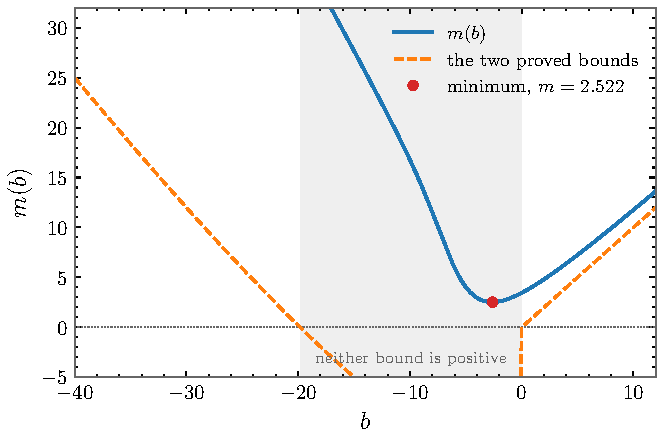
\includegraphics[width=0.72\textwidth]{figures/fig-m-of-b.pdf}
  \caption{The two lower bounds of \Cref{prop:coercivity}, $m(b)\ge b$ for
    $b\ge0$ and \eqref{eq:tail} for $b<0$, shown as dashed lines. They are
    positive outside the shaded interval, which confines any minimizer to a
    compact set; inside it, positivity comes from \Cref{thm:positivity}, which
    is independent of $b$. The solid curve is $m$ itself, obtained by
    diagonalizing $h_b$ in a harmonic-oscillator basis; it is drawn for
    orientation only and no statement in this paper depends on it.}
  \label{fig:m}
\end{figure}

\section{The minimum and the critical coupling}
\label{sec:min}

\begin{proof}[Proof of \Cref{thm:main}]
  Continuity is \Cref{prop:continuity}, positivity is
  \Cref{thm:positivity}, and $m(b)\to+\infty$ as $|b|\to\infty$ is
  \Cref{prop:coercivity}. For the last assertion, choose $R>0$ so large that
  $m(b)>m(0)$ whenever $|b|>R$, which \Cref{prop:coercivity} permits. The
  restriction of $m$ to the compact interval $[-R,R]$ is continuous and
  therefore attains a minimum at some $b_*\in[-R,R]$, and
  $m(b_*)\le m(0)<m(b)$ for every $|b|>R$, so $b_*$ minimizes $m$ over
  $\mathbb R$. Positivity at $b_*$ is \Cref{thm:positivity}.
\end{proof}

\begin{proof}[Proof of \Cref{cor:lambda}]
  By \cite{baez1992renormalized}, solutions at coupling $\lambda>0$ correspond
  one to one with the real $b$ satisfying $m(b)=\lambda^{-2/3}$. By
  \Cref{thm:main} the range of $m$ is contained in $[m_0,\infty)$ with
  $m_0>0$, and, $m$ being continuous with $m(b)\to+\infty$ at both ends and
  attaining $m_0$, its range is exactly $[m_0,\infty)$. Hence
  $m(b)=\lambda^{-2/3}$ has a solution if and only if
  $\lambda^{-2/3}\ge m_0$, that is, if and only if $\lambda\le m_0^{-3/2}$.
\end{proof}

\section{What is not proved}
\label{sec:remarks}

\Cref{thm:main} gives the existence of a minimizer and the strict positivity
of the minimum value. It does not give uniqueness of the minimizer, and it
does not address the separate conjecture of \cite{baez1992renormalized} that
$m$ has exactly one critical point; that question is a level set of
$\lambda_1''$ under the dilation, and is not settled by
\cite{helffer2024critical}, which settles the zeros of $\lambda_1'$.

Neither does the theorem give a numerical enclosure. The proof of
\Cref{thm:positivity} bounds $m(b)$ below by $2\delta(b)\|pG_b\|^2$, and both
factors are accessible in principle; combined with the analytic dependence of
the family on $b$ and with interval arithmetic, this route would give certified
rational-endpoint bounds for $m_0$, and hence for
$\lambda_c=m_0^{-3/2}$. That is not attempted here.

\section*{Acknowledgments}

Z.\ Y.\ acknowledges support from the Strategic Priority Research Program of the
Chinese Academy of Sciences under Grant No.~XDB1680102. Z.\ Y.\ also
acknowledges support by National Natural Science Foundation of China (Grant
No.~12247101). We also acknowledge Gewu Intelligence Lab for providing the
collaborative research environment in which this project was developed.

Large language models were used substantively in this work: OpenAI GPT-5.6 Sol
in solving the problem, including the formulation of arguments and the
derivation of intermediate steps, and Anthropic Claude Opus~5 in surveying the
literature and in drafting and revising the manuscript. The author specified
the problem, guided the approach to be taken, checked every argument and
result they produced, and takes full responsibility for the content of this
manuscript.

\bibliographystyle{amsplain}
\bibliography{references,unverified}

\end{document}
